\paragraph{Алгоритм Диница}

\begin{definition}
    Алгоритм Диница.

    Проведём  bfs , оставим только те  рёбра, которые лежат на кратчайших путях (с меньшего на больший слой). Уберём все тупики.

    Найдём так кратчайший путь (идём по любому ребру), запустим на нём поток величины равной минимальной пропускной способности на пути. 
    Таким образом хотя бы одно из рёбер уйдёт. Повторим. Остановимся когда $s$ станет тупиком.
        
\end{definition}

\begin{center}
    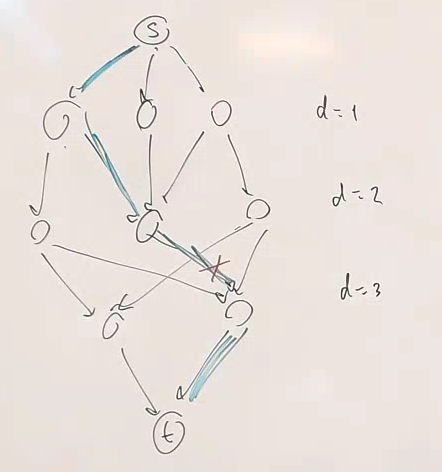
\includegraphics[scale=0.7]{img/dinitsa_algoritm}    
\end{center}

\begin{lstlisting}[mathescape=true]
    while есть путь $s\to t$:
        bfs()
        while dfs():
            $\Delta = \min$
            f += $\Delta$
            удалить тупики 
    (можно удалять лениво: 
        если dfs не смог дойти до t, 
        возвращаемся из рекурсии и 
        убираем за собой ребро)
\end{lstlisting}

Внешний $while$ выполняется не больше $n$ раз. Внутренний не больше $m$. 
Суммарная асимптотика: $\mathcal{O}(n^2m)$. $n$ на каждый $dfs$. Удаление тупиков -- суммарно $n$, не страшно.

Если добавить масштабирование, то асимптотика станет $\mathcal{O}(nm \ln C)$

\paragraph{Алгоритм Гольберга-Торьяна}
План: не терять все пути, которые мы нашли раньше.

\begin{enumerate}
    \item Нашли какой-то кратчайший путь
    \item Нужно найти на нём минимальное $\p C$, только значение.
    \item Прибавить этот $\p C$ ко потоку 
    \item Нужно найти минимальное ребро, чтобы его убрать.
    \item Помним предыдуший путь. На нём есть ребро идущее в тупик. Уберём его. Будем делать так пока таких не будет, а тогда мы сможем пройти в $t$. 
    \item В целом будем идти до ближайшего осколка предыдущего пути.
    \item Из этих путей будем дерево.
\end{enumerate}

План закончился, теперь алгоритм:
\begin{enumerate}
    \item У каждой вершины будет не более одного исходящего ребра -- дерево.
    \item $s$ принадлежит дереву. Пойдём по помеченным рёбрам, пока не упёрлись. Дошли до корня дерева $s$.
    \item Если дошли до $t$ -- радуемся и на этом пути делаем все действия (минимальная пропускная спосность, ко всем на пути прибавляем $\Delta$, убираем минимальные)
    \item Если не дошли -- идём куда-нибудь. Идём до корня уже той вершины. Заодно помечаем ребро п которому мы ``куда-нибудь'' перешли. Повторяем.
\end{enumerate}

Псевдо-псевдо-кот:
\begin{lstlisting}[mathescape=true]
    while есть путь $s \to t$:
        bfs()
        while не удалили $s$:
            v = root(s)
            if v == t:
                $\Delta$, e = min(s..v)
                add(s..v, -\Delta)
                cut(e)
            else:
                if v -- тупик:
                    for all wv:
                        cut(wv)
                else:
                    (vu) -- любое ребро (d(u) = d(v) + 1)
                    link(vu)       
\end{lstlisting}

\begin{itemize}
    \item Большоой while -- $n$ раз
    \item bsf -- $m$
    \item корень суммарн $m\ln n$. Каждый if тоже $m\ln n$
\end{itemize}

Время работы алгоритма~--- $\mathcal{O}\left( nm \ln n \right) $.

\paragraph*{Алгоритм Малхотры -- Кумара -- Махешвари}

Идея: удалять за раз не ребро, а целую вершину. Какую вершину проще всего удалить? У которой минимальная пропускная способность\ldots

$c(v) = \min \left( \sum c_{uv}, \sum c_{uw} \right) $

\begin{enumerate}
    \item Берём вершину. Течём из неё по одному ребру. Если не хватает, пихаем сколько получится. Пихаем в другие, чтобы в сумме было $\Delta$/
    \item Повторяем на вершинах ниже.
    \item От $s$ делаем по обратным рёбрам.
\end{enumerate}

Время работы алгоритма~--- $\mathcal O(n\cdot (n\cdot n + m)) = O(n^3)$
\endinput